Una vez que demostramos tanto la correctitud como la complejidad temporal de nuestro algoritmo, pasamos a la fase de experimentación. En esta sección vamos a comprobar empíricamente que nuestro algoritmo tiene una complejidad temporal de $O(n^3)$, así como también mostrar como resolvemos algunos casos interesantes.

En este primer caso utilizamos instancias aleatorias, con distintos $n$ (es decir, variando en la cantidad total de cartas).

\begin{figure}[H]
  \begin{minipage}{0.5\linewidth}
    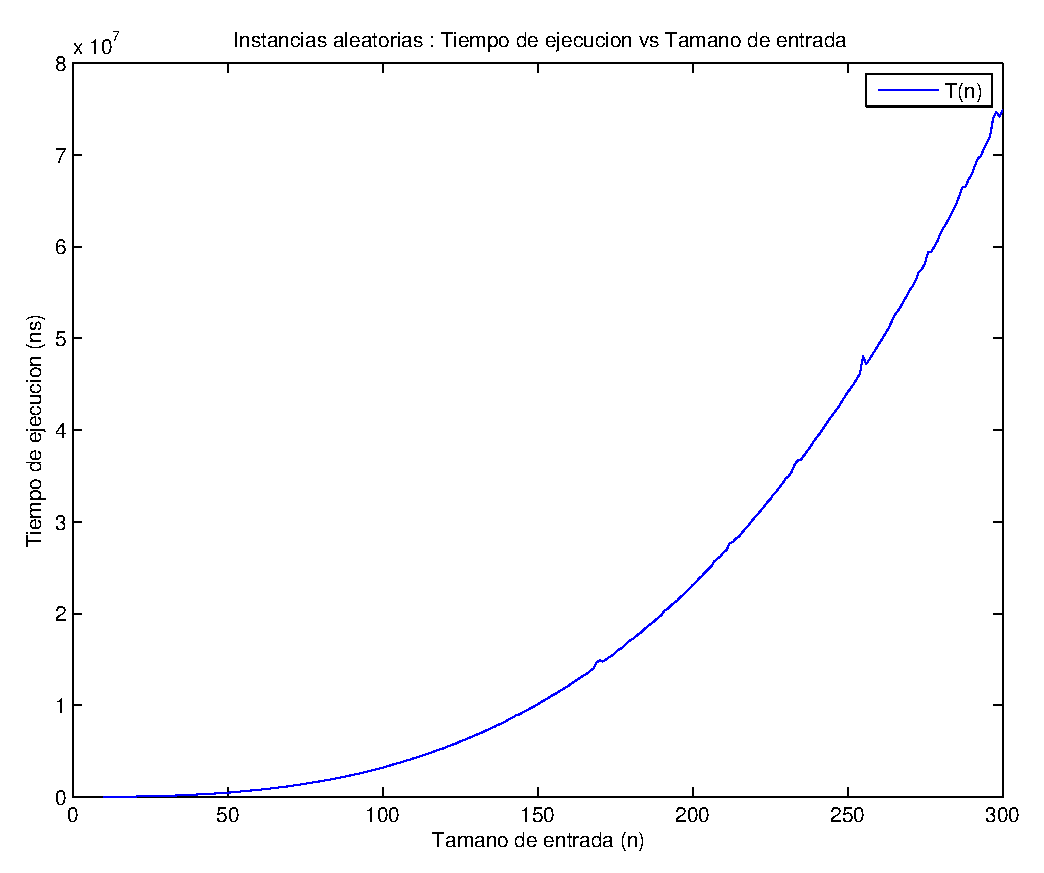
\includegraphics[width=\linewidth]{img/problema1/instancia_aleatoria.eps}
    \caption{Tiempo de ejecución instancia aleatoria}\label{fig:problema1-aleatoria}
  \end{minipage}
  \hfill
  \begin{minipage}{0.5\linewidth}
    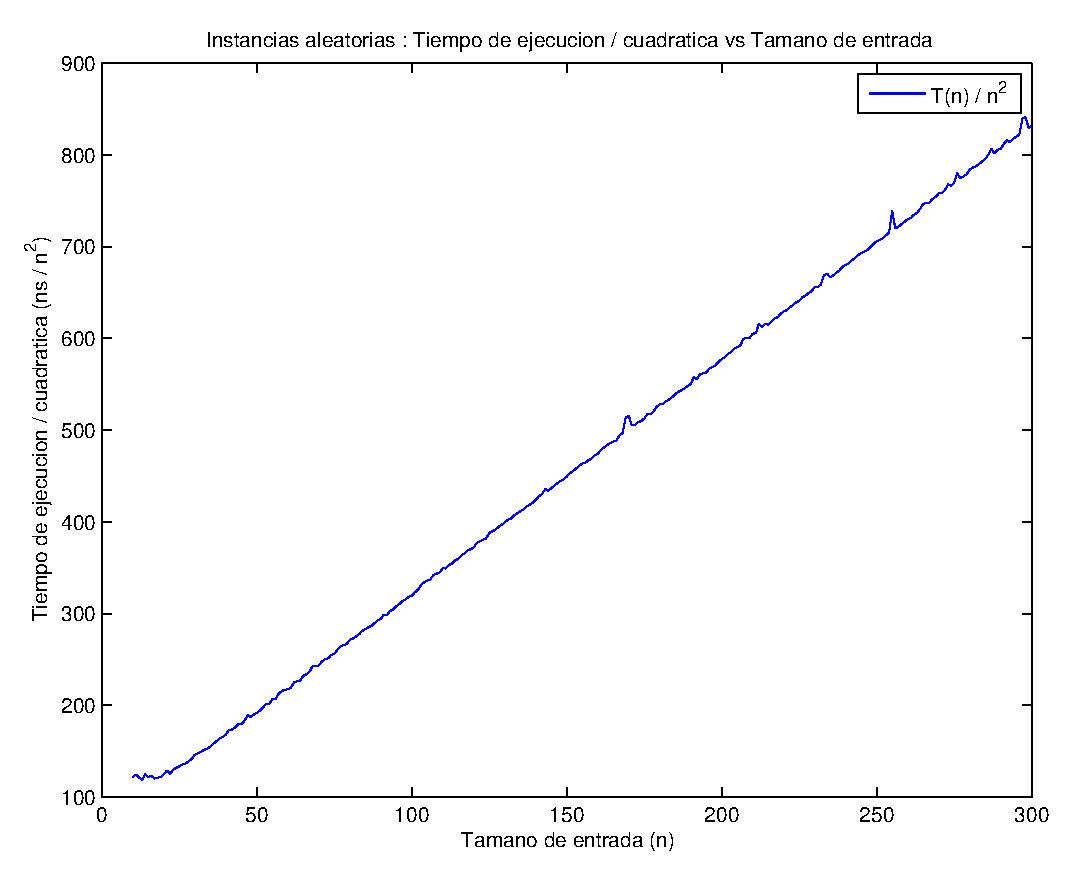
\includegraphics[width=\linewidth]{img/problema1/instancia_aleatoria_div_n2.eps}
    \caption{Idem, dividido por $n^2$}\label{fig:problema1-aleatoria-n2}
  \end{minipage}
\end{figure}

En la figura \ref{fig:problema1-aleatoria} no podemos notar la complejidad temporal de la función. Por esto, dividimos por $n^2$ y plasmamos ese resultado en la figura \ref{fig:problema1-aleatoria-n2}. En esta última figura, vemos claramente que $T(n) / n ^ 2$ es una recta. De esta manera, pudimos comprobar empíricamente que $T(n)$ tiene una complejidad temporal de $O(n^3)$, lo cual demostramos anteriormente. En la figura \ref{fig:problema1-aleatoria-n2} podemos observar unos picos pequeños. Luego de realizar la experimentación, deducimos que dichos picos existen debido al desalojo por parte del \emph{scheduler}.

Luego de mostrar qué es lo que ocurre con instancias aleatorias y ver que pasa en el caso promedio, intentamos analizar el mejor y peor caso de este algoritmo. Luego de analizarlo, llegamos a la conclusión de que este algoritmo nunca va a tardar menos de $O(n^3)$ pasos, ya que nuestro algoritmo debe completar la matriz en su totalidad. Esto sucede porque nuestro algoritmo debe verificar todas las posibilidades que nos ofrece el juego para jugar de la manera óptima. Si el algoritmo no completara algunos casilleros de la matriz estaría observando tan sólo un subconjunto de los posibles movimientos del juego, y de esta forma sería muy posible que llegue a una solución que no sea óptima.

En la sección \ref{problema1-complejidad} demostramos que nuestro algoritmo tiene una complejidad temporal de $O(n^3)$. Por otro lado, también tiene una complejidad de $\omega(n^3)$, ya que siempre debe al menos llenar todas las casillas y al llenar cada casilla se tiene una complejidad lineal. Por lo tanto, al ser $O(n^3)$ y $\omega(n^3)$, podemos decir que la complejidad es de $\theta(n^3)$.

De esta forma, no vamos a incluir casos de ``mejor caso'' o ``peor caso'' ya que nuestro algoritmo siempre tiene complejidad cúbica.